% ======================================================================
\section{Numerical illustrations}\label{sec:experiments}
% ======================================================================

The experiments below illustrate the theorems; they are not needed for the proofs. All of
them run Algorithm~1 in heavy-ball form (the implementation in
\texttt{experiments/common.py} is a direct transcription of the update
$v_{k+1}=\beta v_k-\alpha_kg_k$, $x_{k+1}=x_k+v_{k+1}$), vectorized over independent runs;
expectations are estimated by averaging over runs. Every figure is produced by one script
(\cref{app:reproduce}).

\paragraph{Test problems.}
\begin{enumerate}[label=(P\arabic*)]
\item \emph{Quadratic:} $f(x)=\frac h2x^2$ with $h=L=1$; stochastic gradient
  $g=hx+\xi$, $\xi\sim\mathcal N(0,\sigma^2)$.
\item \emph{Nonconvex PL function:} $f(x)=\sum_{i=1}^{10}(x_i^2+3\sin^2x_i)$ on $\R^{10}$
  ($L=8$, $\mu=\frac1{32}$, $\fs=0$, \cref{lem:pl-facts}(c)); stochastic gradient
  $g=\nabla f(x)+\xi$ with $\xi\sim\mathcal N(0,\frac{\sigma^2}{10}I)$, so that
  $\E\norm{\xi}^2=\sigma^2$.
\item \emph{Nonconvex logistic regression:}
  $f(x)=\frac1n\sum_{i=1}^n\log\bigl(1+e^{-b_ia_i^\top x}\bigr)+\lambda\sum_{j=1}^d\frac{x_j^2}{1+x_j^2}$
  with $n=1000$, $d=20$, $\lambda=0.1$, features $a_i\sim\mathcal N(0,I_d)$, and labels
  $b_i\in\{\pm1\}$ drawn from the logistic model with a random parameter vector. The
  regularizer is nonconvex. Stochastic gradients use one uniformly sampled example (mini-batch
  size $1$); they are unbiased with bounded variance, and $f$ is $L$-smooth with
  $L\le\frac{\norm{A}_2^2}{4n}+2\lambda\approx0.515$, where $A$ has rows $a_i^\top$. All runs start
  at $x_0=(-1,\dots,-1)$.
\item \emph{The function of \cref{ex:lrp}} (strongly convex, exact gradients).
\end{enumerate}

\paragraph{Potential versus function value (\cref{fig:potential}).} On (P1) with $\beta=0.9$
and the largest step allowed by \cref{thm:master}, $\alpha=(1-\beta)^2/(2L)=0.005$, the
function value $f(x_k)$ is not monotone even without noise, because the iterate overshoots
(panel (b)); the potential $\Phi_k$ decreases at every step, as guaranteed by
\cref{cor:when-decrease}. (The script also checks this monotonicity numerically.) With noise
(panel (c)), the empirical floor of $\E f(x_k)$ is $0.01252$, matching the exact value of
\cref{prop:noise-floor} to four digits.

\begin{figure}[t]
\centering
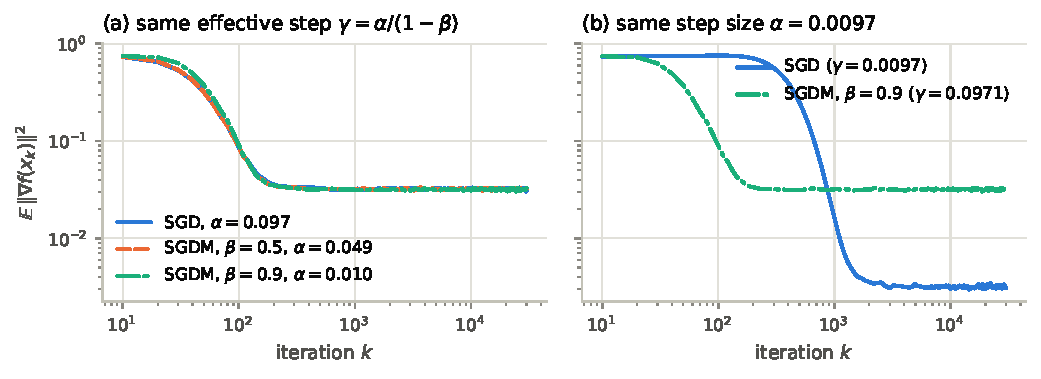
\includegraphics[width=\textwidth]{figures/sgd_vs_sgdm.pdf}
\caption{SGD versus SGDM on the nonconvex logistic regression problem (P3), mean of
$\norm{\nabla f(x_k)}^2$ over $100$ runs (lightly smoothed). (a)~Same effective step
$\gamma=\frac{1-0.9}{2L}$, inside the range of \cref{thm:master} for every $\beta$ shown: the
three methods are indistinguishable. (b)~Same raw step $\alpha=\frac{(1-0.9)^2}{2L}$:
momentum $\beta=0.9$ makes the effective step $10$ times larger, so it converges faster at
first but stalls at a $10$ times higher noise floor.}
\label{fig:sgd-vs-sgdm}
\end{figure}

\paragraph{SGD versus SGDM (\cref{fig:sgd-vs-sgdm}).} On (P3), SGD and SGDM with
$\beta\in\{0.5,0.9\}$ run at the same effective step size produce practically identical
curves (panel (a)), including the level of the noise floor: SGDM behaves like SGD with step
$\gamma$, as the parallel between \cref{lem:sgd-step} and \cref{thm:master} suggests. At
the same raw step size (panel (b)), momentum is simply a ten times larger step: faster
initial progress, ten times higher floor, consistent with \cref{prop:noise-floor}.

\begin{figure}[t]
\centering
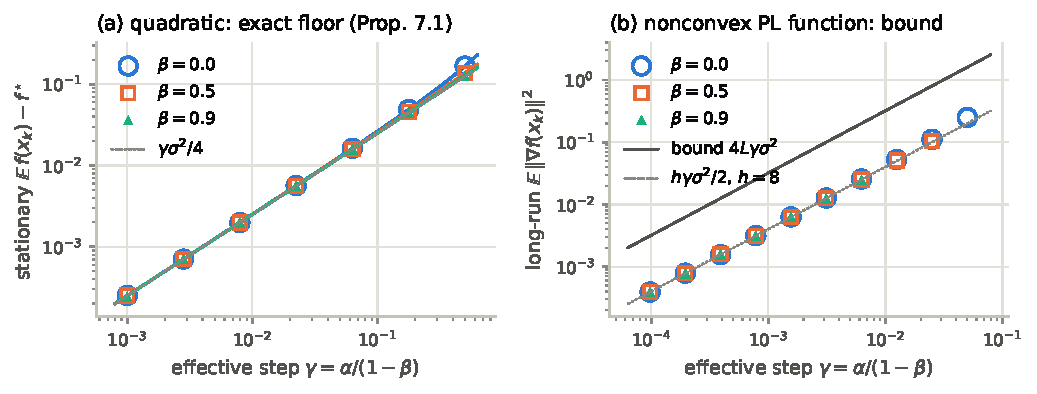
\includegraphics[width=\textwidth]{figures/noise_floor.pdf}
\caption{The noise floor with a constant step scales like $\gamma\sigma^2$ and, to first
order, depends on $(\alpha,\beta)$ only through $\gamma$ (markers for different $\beta$ lie
on top of each other). (a)~Quadratic (P1), $\sigma=1$: empirical stationary $\E f(x_k)$
(markers; $4000$ runs) and the exact formula \eqref{eq:noise-floor} (lines). (b)~Nonconvex
PL function (P2), $\sigma=1$: long-run $\E\norm{\nabla f(x_k)}^2$ ($400$ runs) for step
sizes inside the range of \cref{thm:master}, the bound $4L\gamma\sigma^2$ of
\cref{thm:nonconvex} (as $K\to\infty$), and the local quadratic prediction
$h\gamma\sigma^2/2$ with $h=f''(0)=8$.}
\label{fig:noise-floor}
\end{figure}

\paragraph{The noise floor (\cref{fig:noise-floor}).} For each $\beta\in\{0,0.5,0.9\}$ and a
range of effective step sizes we run the method from the minimizer until it reaches
stationarity and average the quantity of interest over time and runs. On the quadratic,
the measurements agree with \eqref{eq:noise-floor} to within $2\%$ for every $(\gamma,\beta)$.
On the nonconvex PL function, the measured floors lie on the line $h\gamma\sigma^2/2$
predicted by the local quadratic approximation at the minimizer, and about a factor $8$
below the bound $4L\gamma\sigma^2$ of \cref{thm:nonconvex}: the theorem has the correct
dependence on $\gamma$ and $\sigma$, with a pessimistic constant. In both panels the points for
different $\beta$ coincide.

\begin{figure}[t]
\centering
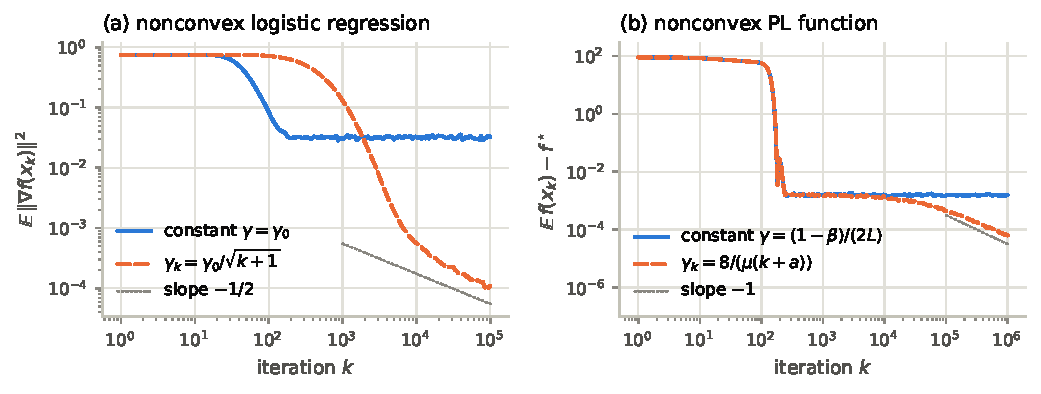
\includegraphics[width=\textwidth]{figures/diminishing.pdf}
\caption{Diminishing step sizes remove the noise floor ($\beta=0.9$; both schedules start
from the same $\gamma_0=\frac{1-\beta}{2L}$). (a)~Nonconvex logistic regression (P3), $50$ runs:
constant step versus $\gamma_k=\gamma_0/\sqrt{k+1}$ (\cref{thm:diminishing}(c)). (b)~Nonconvex
PL function (P2), $100$ runs: constant step versus $\gamma_k=\frac8{\mu(k+a)}$ with
$a=\frac{16L}{\mu(1-\beta)}$ (\cref{cor:pl-decay}); the dotted lines have slopes $-\frac12$ and
$-1$.}
\label{fig:diminishing}
\end{figure}

\paragraph{Diminishing steps (\cref{fig:diminishing}).} With a constant step the error
stalls at its noise floor; with the schedules of \cref{thm:diminishing,cor:pl-decay} it keeps
decreasing. On the logistic problem the gradient norm decreases roughly like $k^{-1/2}$,
which is the order of $\gamma_k$; on the PL function the optimality gap eventually decreases
like $1/k$, as predicted by \cref{cor:pl-decay}. (The theoretical schedule for the PL function
starts slowly because the certified PL constant $\mu=\frac1{32}$ is much smaller than the
local curvature at the minimizer.) Note also the non-monotone transient around $k\approx200$
in panel (b), another manifestation of overshooting.

\paragraph{The counterexample (\cref{fig:lrp}).} On the function of \cref{ex:lrp},
quadratic-optimal parameters lead to the predicted $3$-cycle, while the step sizes allowed by
\cref{prop:energy} and \cref{thm:master} converge. The script verifies the cycle in exact
rational arithmetic.
